\documentclass[10 pt,usenames,dvipsnames, oneside]{article}
\usepackage{../../../modelo-ensino-medio}



\begin{document}

\begin{center}
  \begin{minipage}[l]{3cm}

\includegraphics[width=2cm]{logo}    
\end{minipage}\hfill
\begin{minipage}[r]{.8\textwidth}
 {\Large \scshape Atividade: Escada Infinita}  
\end{minipage}
\end{center}
\vspace{.2cm}

\ifdefined\prof
%Habilidades da BNCC
\begin{objetivos}
\item \textbf{EM13MAT508} Identificar e associar progressões geométricas (PG) a funções exponenciais de domínios discretos, para análise de propriedades, dedução de algumas fórmulas e resolução de problemas.
\end{objetivos}

%Caixa do Para o Professor
\begin{goals}
%Objetivos específicos
\begin{enumerate}
\item Deduzir uma expressão para a soma dos termos de uma PG infinita.

\end{enumerate}

\tcblower

%Orientações e sugestões
\begin{itemize}
\item O item \titem{f)} envolve uma demonstração. Caso os estudantes encontrem alguma dificuldade, considere fazer a discussão dos itens anteriores e resolva este último item juntamente com eles, conectando com ideias que eles desenvolveram.
\end{itemize}
\end{goals}

\bigskip
\begin{center}
{\large \scshape Atividade}
\end{center}
\fi

Na figura abaixo, os ângulos indicados são retos, $AB$ mede $1$, $BC=CD=q<1$. 

\begin{figure}[H]
\centering
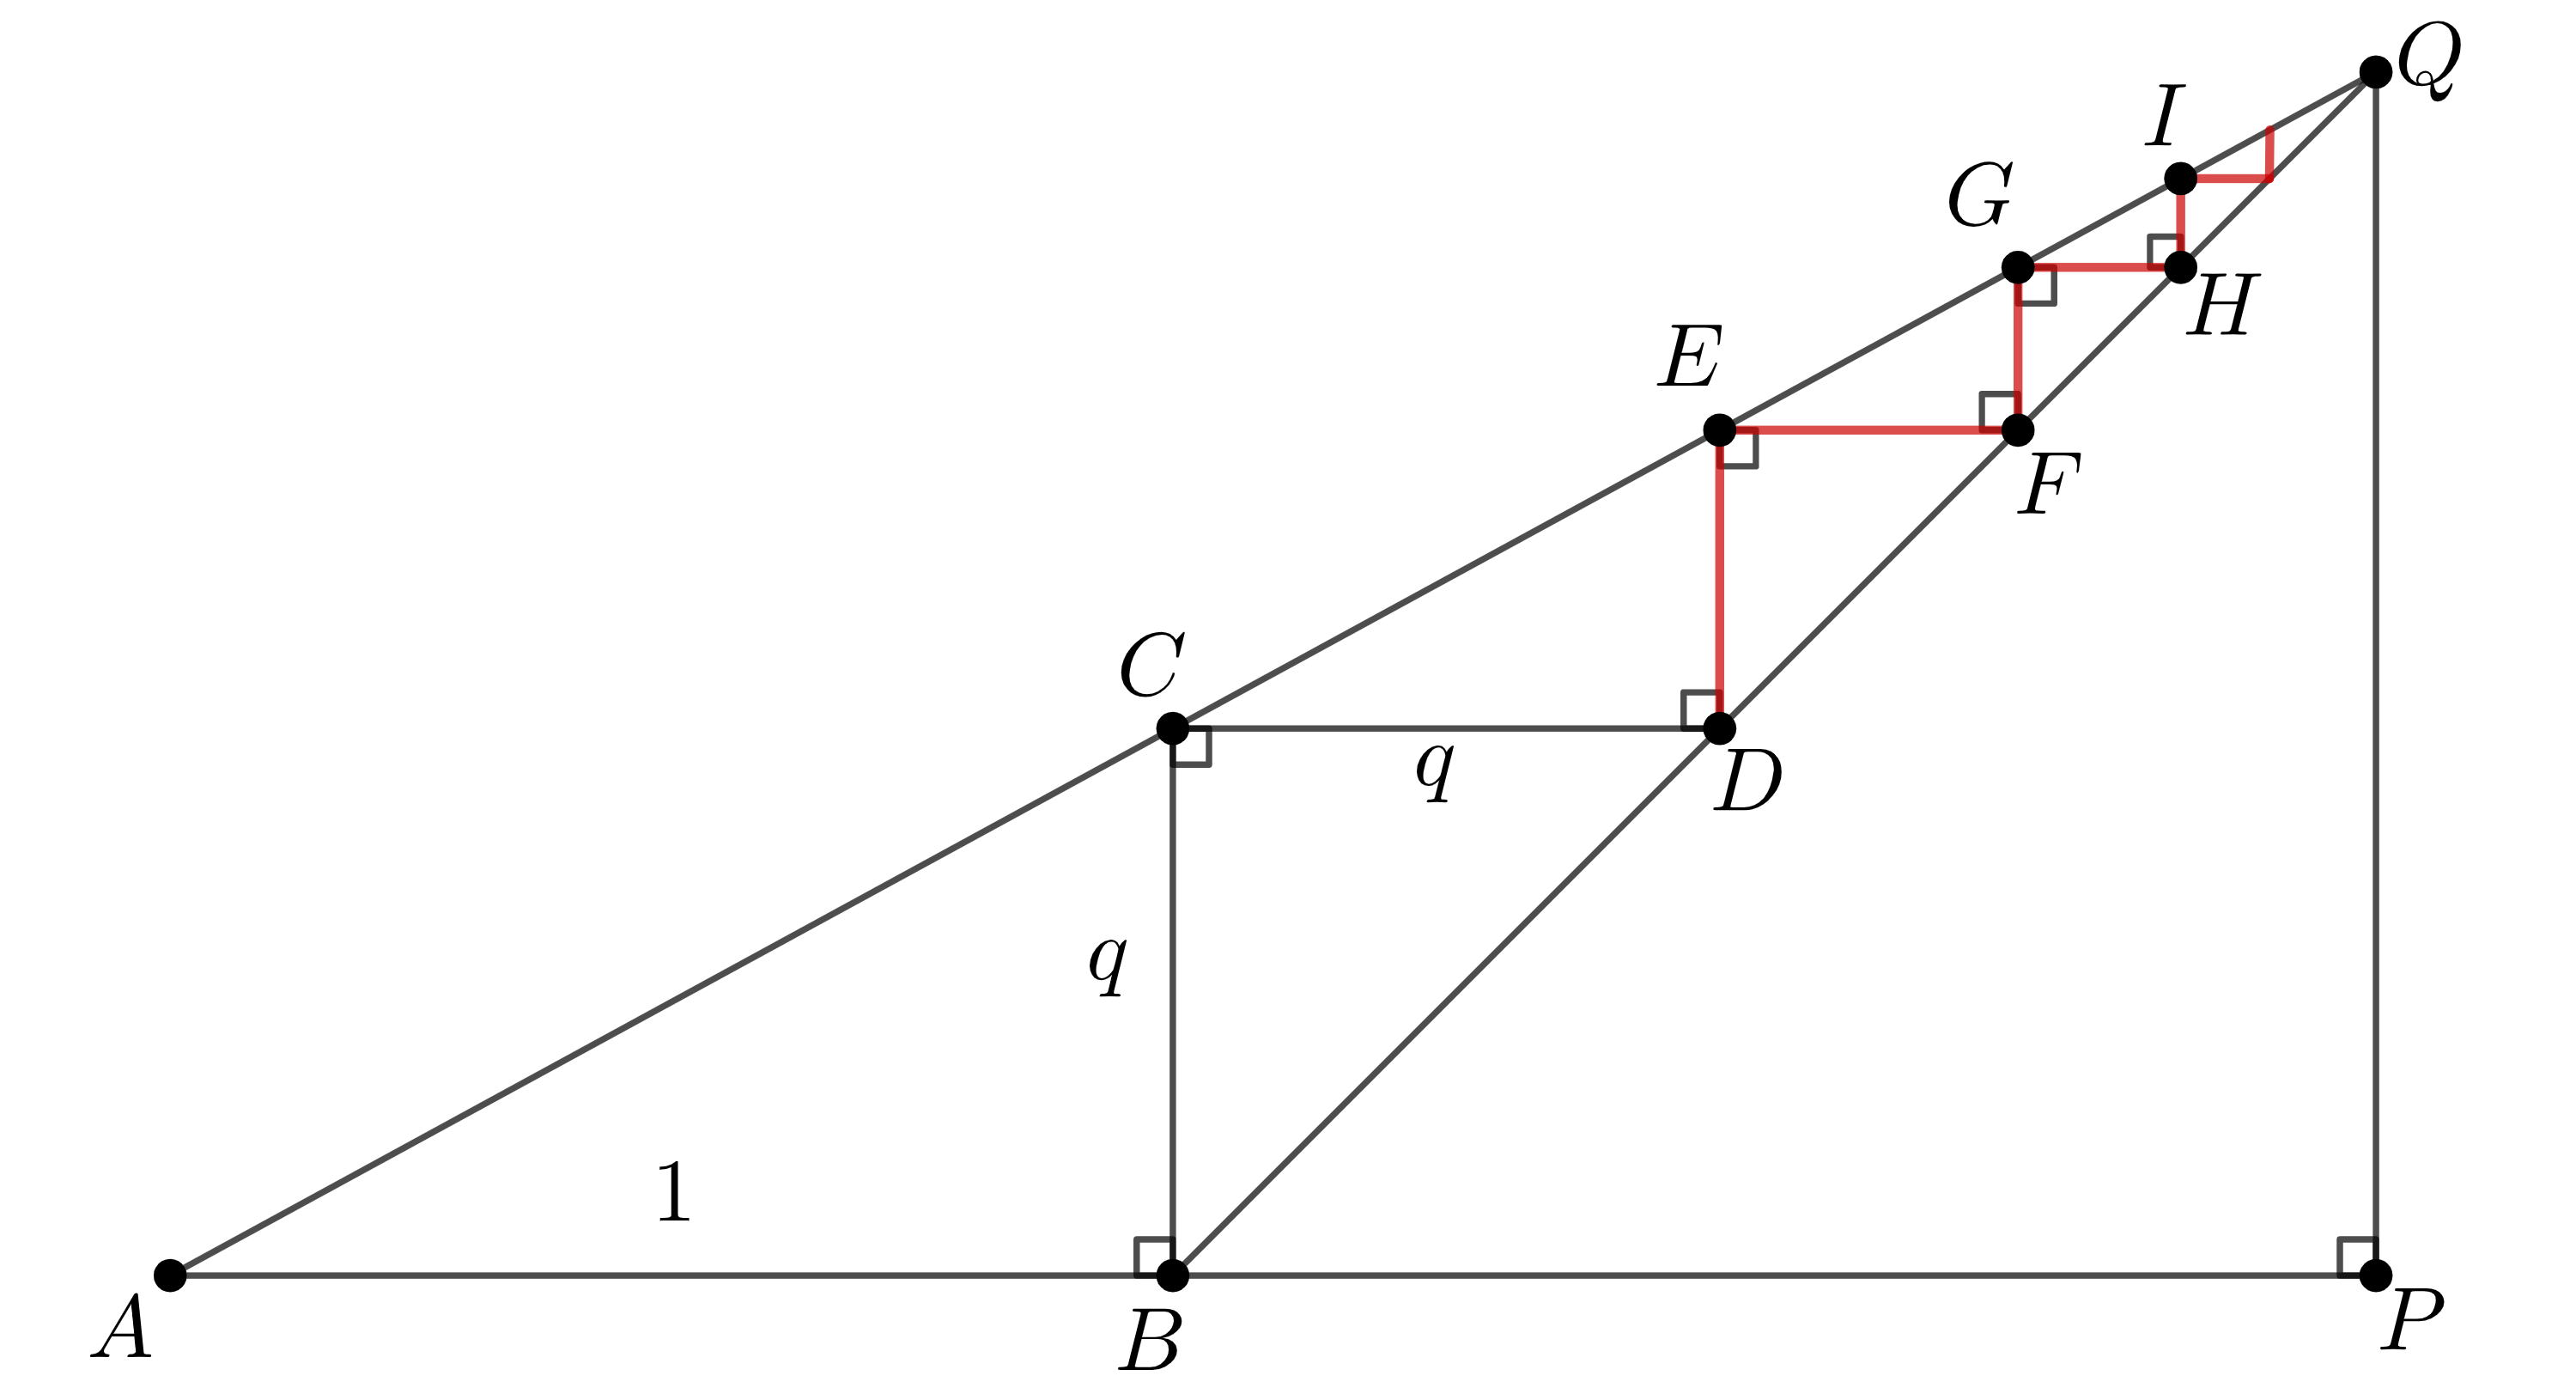
\includegraphics[width=250bp]{escada.png}
\end{figure}

\begin{enumerate}

\item{}
Calcule, em função de $q$, os comprimentos de $DE$, $EF$, $FG$, $GH$ e $HI$.

\item{}
Quais são as sequências de segmentos cujas medidas formam progressões geométricas?

\item{}
Se a construção continuasse indefinidamente, quais seriam as medidas dos novos segmentos horizontais (paralelos a AP)? Que segmento da figura tem comprimento igual à soma de todos os (infinitos) segmentos horizontais? 

\item{}
Por que podemos afirmar que $AP= PQ +1$?

\item{}
Por que podemos afirmar que $PQ=q . AP$?

\item{}
Conclua que a soma de todos os infinitos segmentos horizontais é igual a  $\dfrac{1}{1-q}$.

\end{enumerate}

\ifdefined\prof
\begin{solucao}

\begin{enumerate}
\item $DE=EF=q^2$, $FG=GH=q^3$, $HI=q^4$
\item $(AB, CD, EF, GH)$, $(BC, DE, FG, HI)$
\item $q^4, q^5, q^6,... $ a soma de todos seria igual ao comprimento de $AP$.
\item $AP=AB+BP=1+BP$ e $BP=PQ$, pois o triângulo $BPQ$ é isósceles.
\item Pois $APQ$ é semelhante a $ABC$, assim $\dfrac{PQ}{AP}=\dfrac{BC}{AB}=q$.

$ 1+q+q^2+q^3+...= AP $ e $AP= PQ+1 = q\cdot AP +1$, logo $AP-q\cdot AP=1$, o que nos leva a $AP(1-q)=1 \iff AP=\dfrac 1{1-q}$.
\end{enumerate}
\end{solucao}
\fi

\end{document}